\documentclass{article}
\usepackage{hyperref}
\usepackage[UKenglish]{babel}
\usepackage[UKenglish]{isodate}
\usepackage[utf8]{inputenc}
\usepackage{fullpage}

\usepackage{mathtools}
\usepackage{amsthm}
\usepackage{mathrsfs}
\usepackage{amsfonts}
\usepackage{amssymb}
\usepackage{pifont}

\usepackage[linesnumbered,ruled,vlined]{algorithm2e}
\usepackage{tikz}
\usepackage[capitalize]{cleveref}
\usepackage{booktabs}
\usepackage{multirow}
\usepackage{colortbl}

\usetikzlibrary{fit,positioning,trees,cd}
\usetikzlibrary{shapes}
\usetikzlibrary{arrows}
\usetikzlibrary{arrows.meta}

\crefname{algocf}{algorithm}{Algorithms}
\Crefname{algocf}{Algorithm}{Algorithms}

\newtheorem{theorem}{Theorem}
\theoremstyle{definition}
\newtheorem{definition}{Definition}
\newtheorem{example}{Example}
\newtheorem{observation}{Observation}
\theoremstyle{remark}
\newtheorem*{remark}{Remark}

\makeatletter
\newcommand\incircbin
    {%
      \mathpalette\@incircbin
    }
    \newcommand\@incircbin[2]
                          {%
                            \mathbin%
                                {%
                                  \ooalign{\hidewidth$#1#2$\hidewidth\crcr$#1\bigcirc$}%
                                }%
                          }
                          \newcommand{\oland}{\incircbin{\land}}
                          \newcommand{\olor}{\incircbin{\lor}}
                          \newcommand{\Contradiction}{\incircbin{\bot}}
                          \newcommand{\Tautology}{\incircbin{\top}}
                          \newcommand{\Smoothing}{\incircbin{}}
                          \newcommand{\Unit}{\incircbin{1}}
                          \makeatother

\newcommand\pfun{\mathrel{\ooalign{\hfil$\mapstochar\mkern5mu$\hfil\cr$\to$\cr}}}
\newcommand\mdoubleplus{\mathbin{+\mkern-10mu+}}
\newcommand*{\twoheadrightarrowtail}{\mathrel{\rightarrowtail\kern-1.9ex\twoheadrightarrow}}
\newcommand{\cmark}{\ding{51}}%
\newcommand{\xmark}{\ding{55}}%

\DeclareMathOperator{\CR}{\textsc{CR}}
\DeclareMathOperator{\DR}{\textsc{DR}}
\DeclareMathOperator{\IE}{\textsc{IE}}
\DeclareMathOperator{\Reff}{\textsc{Ref}}
\DeclareMathOperator{\wwp}{w}
\DeclareMathOperator{\wwn}{\overline{w}}

\DeclareMathOperator{\dom}{dom}
\DeclareMathOperator{\id}{id}
\DeclareMathOperator{\Imm}{Im}
\DeclareMathOperator{\Doms}{Doms}
\DeclareMathOperator{\size}{\sigma}
\DeclareMathOperator{\Vars}{Vars}
\DeclareMathOperator{\WMC}{WMC}
\DeclareMathOperator{\gr}{gr}

\title{Recursive Solutions to First-Order Model Counting}

\begin{document}
\maketitle

\section{Introduction}

\paragraph{Abstract.} First-order model counting (FOMC) is a #P-complete computational problem that asks to count the models of a sentence in first-order logic. Despite being around for more than a decade, practical FOMC algorithms are still unable to compute functions as simple as a factorial. We argue that the capabilities of FOMC algorithms are severely limited by their inability to express arbitrary recursive computations. To enable arbitrary recursion, we relax the restrictions that typically accompany domain recursion and generalise circuits used to express a solution to an FOMC problem to graphs that may contain cycles. To this end, we enhance the most well-established (weighted) FOMC algorithm ForcLift with new compilation rules and an algorithm to check whether a recursive call is feasible. These improvements allow us to find efficient solutions to counting fundamental structures such as injections and bijections.

\begin{figure}[t]
  \centering
  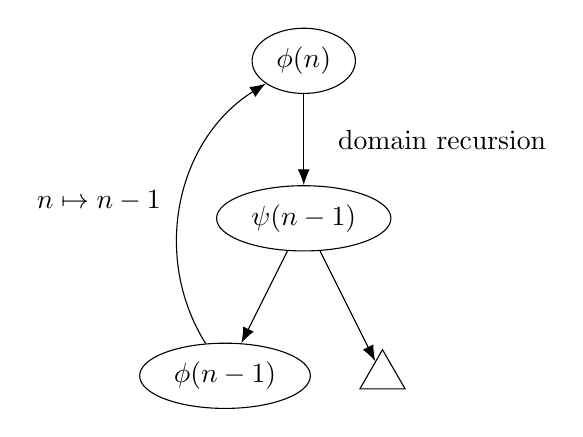
\begin{tikzpicture}[triangle/.style = {regular polygon, regular polygon sides=3}]
    \node[draw,ellipse] (a) at (0, 0) {$\phi(n)$};
    \node[draw,ellipse] (b) at (0, -2) {$\psi(n-1)$};
    \node[draw,ellipse] (c) at (-1, -4) {$\phi(n-1)$};
    \node[draw,triangle] (d) at (1, -4) {};
    \draw[-{Latex[length=2mm]}] (a) -- (b) node [midway,xshift=50] {domain recursion};
    \draw[-{Latex[length=2mm]}] (b) -- (c);
    \draw[-{Latex[length=2mm]}] (b) -- (d);
    \draw[-{Latex[length=2mm]}] (c) to [bend left=45] node [midway,xshift=-30] () {$n \mapsto n-1$} (a);
  \end{tikzpicture}
  \caption{An illustration of the main idea.}
  \label{fig:idea}
\end{figure}

In a way, we're dividing the idea of domain recursion between the IDR and the Ref nodes, thus also generalising it. [TODO: mention \cref{fig:idea}.]

\section{First-Order Logic}

In this section, we describe a variation of function-free first-order logic with equality. For a more complete exposition of first-order logic, see the book by \cite{DBLP:books/daglib/0023546}.

In first-order logic, an \emph{atom} (i.e., an atomic formula) is either $t_1 = t_2$ or $P(t_1, \dots, t_n)$ for some predicate $P$ and terms $(t_i)_{i=1}^n$. Here, $n \in \mathbb{N}_0$ is the \emph{arity} of $P$. A \emph{term} is either a constant or a variable (we also call terms \emph{arguments}). An atom is \emph{ground} if all of its terms are constants.

A \emph{formula} is a well-formed expression that connects atoms using the previously described logical operators as well as universal ($\forall x \in D. \phi$) and existential ($\exists x \in D. \phi$) quantifiers. Here, $x$ is a variable, $D$ is a domain, and $\phi$ is a formula. A variable occurrence is \emph{bound} if it is within the scope of a quantifier for that variable, otherwise it is \emph{free}. A formula is a \emph{sentence} if all of its variable occurrences are bound.\footnote{In the rest of this chapter, all formulas in first-order logic are assumed to be sentences.}

\subsection{How to Interpret a Sentence}

Let $\phi$ be a sentence. Since each variable in $\phi$ is introduced by a quantifier, each variable is linked to a unique domain. As is done implicitly in previous work \citep{DBLP:phd/basesearch/VandenBroeck13}, we make the following assumption.

\begin{assumption}
  Each constant can be mapped to a domain, and each $n$-ary predicate can be mapped to a sequence of $n$ domains such that:
  \begin{enumerate}
  \item ...
  \item ...
  \end{enumerate}
\end{assumption}

First, we assume that each $n$-ary predicate can be associated with a sequence of $n$ domains, one for each of its terms. Second, we assume that each constant can be similarly linked to a unique domain. Third, we assume that equality is only checked between terms that have the same domain.

TODO: describe this more formally. Maybe just two rules: whenever two terms are compared, they have the same domain, the domain of a term is always the same as the $k$-th domain of the predicate.

\begin{itemize}
\item Interpretation
  \begin{itemize}
  \item domains as sets
  \item constants as specific elements of domains (different constant implies different element. If the domain is not big enough, then the formula is unsat.)
  \item variables (indicated during quantification)
  \item predicates are interpreted as relations
  \end{itemize}
\item models are defined very differently: all combinations of relations that satisfy the sentence.
\item (multiple) (finite) domains (of discourse). This makes, e.g., satisfiability decidable and a FO formula can always be expanded to a propositional one.
\end{itemize}

more on first-order logic: \citep{DBLP:books/daglib/0023546}. The MLN paper also has a description

\section{Preliminaries}

\paragraph{Things I might need to explain.}
\begin{itemize}
\item atom, (positive/negative) literal, constant, predicate, variable, clause, unit clause, first-order logic
\item $\WMC$, $\wwp$, $\wwn$.
\item two parts: compilation and inference.
\item During inference, there is a domain size map $\size\colon \mathcal{D} \to \mathbb{N}_0$.
\item mention which rules are in $\Gamma$ and which ones are in $\Delta$ (and why tryCache has to be in $\Delta$). TODO: having notation for $\Delta$ and $\Gamma$ isn't that necessary
\item My formalisation of constraints is more restrictive than the original (e.g., in the thesis).
\item \textsc{ForcLift}
\item $\sqcup$ for both sets and functions
\end{itemize}

TODO: reorder Section 6 to introduce DR before CR before Ref.

\paragraph{Notation.}
\begin{itemize}
\item We write $\to$ for functions, $\pfun$ for partial functions, $\twoheadrightarrowtail$ for bijections, and $\hookrightarrow$ for set inclusion. Let $\id$ denote the identity function (on any domain). For any function $f$, let $\Imm f$ be the image of $f$.
\end{itemize}

Most of the definitions here are adaptations/formalisations of \cite{DBLP:conf/ijcai/BroeckTMDR11} and the corresponding code.

\begin{definition}
  A \emph{domain} is a symbol for a finite set.\footnote{In the context of functions, the domain of a function $f$ retains its usual meaning and is denoted $\dom(f)$.}
\end{definition}

\begin{definition}
  An \emph{(inequality) constraint} is a pair $(a, b)$, where $a$ is a variable, and $b$ is either a variable or a constant.
\end{definition}

\begin{definition}
  A \emph{clause} is a triple $c = (L, C, \delta_c)$, where $L$ is a set of literals, $C$ is a set of constraints, and $\delta_c$ is a function that maps all variables in $c$ to their domains such that (s.t.) if $(x, y) \in C$ for some variables $x$ and $y$, then $\delta_c(x) = \delta_c(y)$. Note that for convenience sometimes we write $\delta_c$ for the domain map of $c$ without unpacking $c$ into its three constituents.

  Also, let $\Vars$ be a function that maps clauses and sets of literals and inequalities to the set of variables contained within. In particular, $\Vars(c) \coloneqq \Vars(L) \cup \Vars(C)$.
\end{definition}

A \emph{formula} is a set of clauses. All variables in a clause are implicitly universally quantified (but note that variables are never shared among clauses), and all clauses in a formula are implicitly linked by conjunction. This way, one can read formulas as defined here as sentences in first-order logic.

TODO: Note: we will reuse this several times.
\begin{example} \label{example:first}
  Let $\phi \coloneqq \{\, c_1, c_2 \,\}$ be a formula, where
  \begin{equation} \label{phi1}
    c_1 \coloneqq (\{\, \neg p(X, Y), \neg p(X, Z) \,\}, \{\, (Y, Z) \,\}, \{\, X \mapsto a, Y \mapsto b, Z \mapsto b \,\}),
  \end{equation}
  and
  \begin{equation} \label{phi2}
    c_2 \coloneqq (\{\, \neg p(X, Y), \neg p(Z, Y) \,\}, \{\, (X, Z) \,\}, \{\, X \mapsto a, Y \mapsto b, Z \mapsto a \,\}),
  \end{equation}
  for some predicate $p$, variables $X$, $Y$, $Z$, and domains $a$ and $b$. Then in first-order logic $\phi$ could be read as
  \begin{align*}
    (\forall X \in a. \forall Y \in b. \forall Z \in b. Y \ne Z &\implies \neg p(X, Y) \lor \neg p(X, Z)) \land \\
    (\forall X \in a. \forall Y \in b. \forall Z \in a. X \ne Z &\implies \neg p(X, Y) \lor \neg p(Z, Y)).
  \end{align*}
\end{example}

\paragraph{Hashing.}
We use hash codes to efficiently check whether a recursive relationship between two formulas is plausible. (It is plausible if the formulas are equal up to variables and domains.) The hash code of a clause $c = (L, C, \delta)$ combines the hash codes of the sets of constants and predicates in $c$, the numbers of positive and negative literals, the number of inequality constraints $|C|$, and the number of variables $|\Vars(c)|$. The hash code of a formula $\phi$ combines the hash codes of all its clauses and is denoted $\#\phi$.

\paragraph{Notation for lists.}
Let $\langle\rangle$ and $\langle x \rangle$ denote an empty list and a list with one element $x$, respectively. We write $\in$ for (in-order) enumeration, $\mdoubleplus$ for concatenation, and $|\cdot|$ for the length of a list. Let $h : t$ denote a list with first element (a.k.a. head) $h$ and remaining list (a.k.a. tail) $t$. We also use list comprehensions written equivalently to set comprehensions. For example, let $L \coloneqq \langle 1 \rangle$ and $M \coloneqq \langle 2 \rangle$ be two lists. Then $M = \langle 2x \mid x \in L \rangle$, $L \mdoubleplus M = 1 : \langle 2 \rangle$, and $|M| = 1$.

\section{Generalising Circuits to Labelled Graphs}

A \emph{first-order deterministic decomposable negation normal form computational graph} (FCG) is a (weakly connected) directed graph with a a single source, vertex labels, and ordered outgoing edges.\footnote{Note that imposing an ordering on outgoing edges is just a limited version of edge labelling.} We denote an FCG as $G = (V, s, N^+, \tau)$, where $V$ is the set of vertices, and $s \in V$ is the unique source. Also, $N^+$ is the direct successor function that maps each vertex in $V$ to a \emph{list} that contains either other vertices in $V$ or a special symbol $\star$. This symbol means that the target of the edge is yet to be determined.

Vertex labels consist of two parts: the \emph{type} and the \emph{parameters}. For the main definition, we leave the parameters implicit and let $\tau\colon V \to \mathcal{T}$ denote the vertex-labelling function that maps each vertex in $V$ to its type in $\mathcal{T}$. Most of our list of types $\mathcal{T} \coloneqq \{\, \Smoothing, \Unit, \Tautology, \Contradiction, \oland, \olor, \CR, \DR, \IE, \Reff \,\}$ is as described in previous work \cite{DBLP:conf/nips/Broeck11,DBLP:conf/ijcai/BroeckTMDR11} as well as the source code of \textsc{ForcLift}\footnote{\url{https://dtai.cs.kuleuven.be/drupal/wfomc}} but with one new type $\CR$ and two revamped types $\DR$ and $\Reff$. For each vertex $v \in V$, the length of the list $N^+(v)$ (i.e., the out-degree of $v$) is determined by its type $\tau(v)$.

TODO: conjunctions and disjunctions should be different from set-conjunctions and set-disjunctions.

As in previous work \cite{DBLP:conf/ijcai/BroeckTMDR11}, to describe individual vertices and small (sub)-FCGs, we also use notation of the form, e.g., $\Reff_\rho(v)$. Here, the type of the vertex (e.g., $\Reff$) is `applied' to its direct successors (e.g., $v$) using either function or infix notation and provided with its parameter(s) (e.g., $\rho$) in the subscript. We say that `$G$ is an FCG for formula $\phi$' if two conditions are satisfied. First, the image of $N^+$ contains no $\star$'s. Second, $G$ encodes a function that maps the sizes of the domains in $\phi$ to the WMC of $\phi$ (more on this in \cref{sec:evaluation}).

\paragraph{TODO.}
\begin{itemize}
\item provide a short explanation of the types (emphasising which ones are new/updated). %\footnote{The new (as well as significantly renewed) types in \mathcal{T} are described in subsequent (TODO: which ones?) sections. The meanings of other types are described...}
\item have an example of a simple FCG. Maybe describe the figure from later and move it here.
\end{itemize}

\section{Compilation as Search}

\begin{definition}
  A \emph{state} (of the search for an FCG for a given formula) is a tuple $(G, C, L)$, where:
  \begin{itemize}
  \item $G$ is an FCG (or \texttt{null}),
  \item $C$ is a compilation cache that maps integers to sets of pairs $(\phi, v)$, where $\phi$ is a formula, and $v$ is a vertex of $G$ (which is used to identify opportunities for recursion),
  \item and $L$ is a list of formulas (that are yet to be compiled). (Note that the order is crucial!)
  \end{itemize}
\end{definition}

\begin{definition}
  A (compilation) \emph{rule} is a function that takes a formula and returns a set of $(G, L)$ pairs, where $G$ is a (potentially \texttt{null}) FCG, and $L$ is a list of formulas.

  TODO: Take the example from the AIAI talk.
\end{definition}

We assume that if there is a pair $(\texttt{null}, L)$ in the set returned by a rule, then $|L| = 1$, i.e., the rule transformed the formula without creating any vertices.

\begin{algorithm}[t]
  \caption{The (main part of the) search algorithm}
  \label{alg:search}
  \SetKwProg{Fn}{Function}{:}{}
  \SetKwData{solutions}{solutions}
  \SetKwFunction{applyGreedyRules}{applyGreedyRules}
  \SetKwFunction{applyAllRules}{applyAllRules}
  \SetKwFunction{put}{put}
  \SetKwFunction{get}{get}
  \SetKwFunction{emptyy}{empty}
  \KwIn{a formula $\phi_0$}
  \KwOut{all found FCGs for $\phi_0$ are in the set \solutions}
  $\solutions \gets \emptyset$\;
  $C_0 \gets \emptyset$\;
  $(G_0, C_0, L_0) \gets \applyGreedyRules{$\phi_0$, $C_0$}$\;
  \lIf{$L_0 = \langle\rangle$}{$\solutions \gets \{\, G_0 \,\}$}
  \Else{
    $q \gets \text{an empty queue of states}$\;
    $q.\put{$(G_0, C_0, L_0)$}$\;
    \While{{\bf not} $q.\emptyy{}$}{
      \ForEach{state $(G, C, L) \in \applyAllRules{$q.\get{}$}$}{
        \lIf{$L = \langle\rangle$}{$\solutions \gets \solutions \cup \{\, G \,\}$}
        \lElse{$q.\put{$(G, C, L)$}$}
      }
    }
  }
\end{algorithm}

\begin{algorithm}
  \caption{Functions used in \cref{alg:search} for applying compilation rules}
  \label{alg:apply}
  \SetKwProg{Fn}{Function}{:}{}
  \SetKwData{newStates}{newStates}
  \SetKwFunction{applyGreedyRules}{applyGreedyRules}
  \SetKwFunction{applyAllRules}{applyAllRules}
  \SetKwFunction{applyGreedyRulesToAllFormulas}{applyGreedyRulesToAllFormulas}
  \SetKwFunction{mergeFcgs}{mergeFcgs}
  \SetKwFunction{updateCache}{updateCache}
  \KwData{a set of greedy rules $\Gamma$}
  \KwData{a set of non-greedy rules $\Delta$}
  \Fn{\applyGreedyRules{$\phi$, $C$}}{
    \ForEach{rule $r \in \Gamma$}{
      \If{$r(\phi) \ne \emptyset$}{
        $(G, L) \gets \text{any element of } r(\phi)$\;
        \lIf{$G = {\normalfont \texttt{null}}$}{\Return{\applyGreedyRules{the only element of $L$, $C$}}}
        \Else{
          $(V, s, N^+, \tau) \gets G$\;
          $C \gets \updateCache{$C$, $\phi$, $G$}$\;
          \Return{\applyGreedyRulesToAllFormulas{$G$, $C$, $L$}}\;
        }
      }
    }
    \Return{$({\normalfont \texttt{null}}, C, \langle\phi\rangle)$}\;
  }
  \Fn{\applyGreedyRulesToAllFormulas{$(V, s, N^+, \tau)$, $C$, $L$}}{
    \lIf{$L = \langle\rangle$}{\Return{$((V, s, N^+, \tau), C, L)$}}
    $N^+(s) \gets \langle\rangle$\;
    $L' \gets \langle\rangle$\;
    \ForEach{formula $\phi \in L$}{
      $(G', C, L'') \gets \applyGreedyRules{$\phi$, $C$}$\;
      $L' \gets L' \mdoubleplus L''$\;
      \lIf{$G' = {\normalfont \texttt{null}}$}{$N^+(s) \gets N^+(s) \mdoubleplus \langle\star\rangle$}
      \Else{
        $(V', s', N', \tau') \gets G'$\;
        $V \gets V \sqcup V'$\;
        $N^+ \gets N^+ \sqcup N'$\;
        $N^+(s) \gets N^+(s) \mdoubleplus \langle s' \rangle$\;
        $\tau \gets \tau \sqcup \tau'$\;
      }
    }
    \Return{$((V, s, N^+, \tau), C, L')$}\;
  }
  \Fn{\applyAllRules{$s$}}{
    $(G, C, L) \gets s$\;
    $\phi : T \gets L$\;
    $(G', C', L') \gets \text{a copy of } s$\;
    $\newStates \gets \langle\rangle$\;
    \ForEach{rule $r \in \Delta$}{
      \ForEach{$(G'', L'') \in r(\phi)$}{
        \lIf{$G'' = {\normalfont \texttt{null}}$}{$\newStates \gets \newStates \mdoubleplus \applyAllRules{$(G', C', L'')$}$}
        \Else{
          $(V, s, N^+, \tau) \gets G''$\;
          $C' \gets \updateCache{$C'$, $\phi$, $G''$}$\;
          $(G'', C', L'') \gets \applyGreedyRulesToAllFormulas{$G''$, $C'$, $L''$}$\;
          \lIf{$G' = {\normalfont \texttt{null}}$}{$\newStates \gets \newStates \mdoubleplus \langle(G'', C', L'' \mdoubleplus T)\rangle$}
          \lElse{$\newStates \gets \newStates \mdoubleplus \langle(\mergeFcgs{$G'$, $G''$}, C', L'' \mdoubleplus T)\rangle$}
        }
      }
      $(G', C', L') \gets \text{a copy of } s$\;
    }
    \Return{\newStates}\;
  }
\end{algorithm}

\begin{algorithm}
  \caption{Helper functions used by \cref{alg:apply}}
  \label{alg:helpers}
  \SetKwProg{Fn}{Function}{:}{}
  \SetKwFunction{mergeFcgs}{mergeFcgs}
  \SetKwFunction{updateCache}{updateCache}
  \Fn{\updateCache{$C$, $\phi$, $(V, s, N^+, \tau)$}}{
    \lIf{$\tau(s) = \textsc{Ref}$}{\Return{$C$}}
    \lIf{$\#\phi \not\in \dom(C)$}{\Return{$C \cup \{\, \#\phi \mapsto (\phi, s) \,\}$}}
    \lIf{there is no $(\phi', v) \in C(\#\phi)$ s.t. $v = s$}{$C(\#\phi) \gets (\phi, s) \mdoubleplus C(\#\phi)$}
    \Return{$C$}\;
  }
  \Fn{\mergeFcgs{$G = (V, s, N^+, \tau)$, $G' = (V', s', N', \tau')$, $r = s$}}{
    \lIf{$\tau(r) = \textsc{Ref}$}{\Return{\normalfont \texttt{null}}}
    \ForEach{$t \in N^+(r)$}{
      \If{$t = \star$}{
        replace $t$ with $s'$ in $N^+(r)$\;
        \Return{$(V \sqcup V', s, N^+ \sqcup N', \tau \sqcup \tau')$}\;
      }
      $G'' \gets \mergeFcgs{$G$, $G'$, $t$}$\;
      \lIf{$G'' \ne {\normalfont \texttt{null}}$}{\Return{$G''$}}
    }
    \Return{\normalfont \texttt{null}}\;
  }
\end{algorithm}

TODO: explain the `tail' part of the algorithm, i.e., that the first formula is replaced by some vertices and some formulas. And explain why we don't want to have \textsc{Ref} vertices in the cache.

Note: At the end, \texttt{mergeFcgs} will never return \texttt{null} because there is going to be at least one $\star$ in $G$ and the function will find it.

\section{In-Between Compilation and Inference: Smoothing}

\begin{algorithm}
  \SetKwData{changed}{changed}
  \caption{Propagating atoms for smoothing across the FCG in a way that avoids infinite loops}
  \label{alg:smoothing}
  \KwIn{FCG $(V, s, N^+, \tau)$}
  \KwIn{function $\iota$ that maps vertex types in $\mathcal{T}$ to sets of atoms}
  \KwIn{functions $\{\,f_t\,\}_{t \in \mathcal{T}}$ that take a list of sets of atoms and return a set of atoms}
  \KwOut{function $S$ that maps vertices in $V$ to sets of atoms}
  $S \gets \{\, v \mapsto \iota(\tau(v)) \mid v \in V \,\}$\;
  $\changed \gets \texttt{true}$\;
  \While{\changed}{
    $\changed \gets \texttt{false}$\;
    \ForEach{vertex $v \in V$}{
      $S' \gets f_{\tau(v)}(\langle S(w) \mid w \in N^+(v) \rangle)$\;
      \If{$S' \ne S(v)$}{
        $\changed \gets \texttt{true}$\;
        $S(v) \gets S'$\;
      }
    }
  }
\end{algorithm}

[Insert motivation for smoothing from Section 3.4. of the ForcLift paper.] Originally, smoothing was (and still is) a two-step process. First, atoms that are still accounted for in the circuit are propagated upwards. Then, at vertices of certain types, missing atoms are detected and additional sinks are created to account for them. If left unchanged, the first step of this process would result in an infinite loop whenever a cycle is encountered. \Cref{alg:smoothing} outlines how the first step can be adapted to an arbitrary directed graph.

\section{New Compilation Rules}

Let $\mathcal{D}$ be the set of all domains. Note that this set expands during the compilation.

\subsection{Identifying Possibilities for Recursion}

\subsubsection{Notation}

Let $\Doms$ be a function that maps any clause or formula to the set of domains used within. Specifically, $\Doms(c) \coloneqq \Imm \delta_c$ for any clause $c$, and $\Doms(\phi) \coloneqq \bigcup_{c \in \phi} \Doms(c)$ for any formula $\phi$.

For partial functions $\alpha, \beta\colon A \pfun B$ s.t. $\alpha|_{\dom(\alpha) \cap \dom(\beta)} = \beta|_{\dom(\alpha) \cap \dom(\beta)}$, we write $\alpha \cup \beta$ for the unique partial function s.t. $\alpha \cup \beta|_{\dom(\alpha)} = \alpha$, and $\alpha \cup \beta|_{\dom(\beta)} = \beta$.

For any clause $c = (L, C, \delta_c)$, bijection $\beta\colon \Vars(c) \twoheadrightarrowtail V$ (for some set of variables $V$), and function $\gamma\colon \Doms(c) \to \mathcal{D}$, let $c[\beta, \gamma] = d$ be the clause $c$ with all occurrences of any variable $v \in \Vars(c)$ in $L$ and $C$ replaced with $\beta(v)$ (so $\Vars(d) = V$) and $\delta_d\colon V \to \mathcal{D}$ defined as $\delta_d \coloneqq \gamma \circ \delta_c \circ \beta^{-1}$. In other words, $\delta_d$ is the unique function that makes
\[
\begin{tikzcd}
  \Vars(c) \ar[r, tail, two heads, "\beta"] \arrow[d, swap, "\delta_c"] & V = \Vars(d) \ar[d, dashed, "\exists!\delta_d"] \\
  \Doms(c) \ar[r, swap, "\gamma"] & \mathcal{D}
\end{tikzcd}
\]
commute. For example, if clause $c_1$ is as in \cref{example:first}, then
\begin{multline*}
  c_1[\{\, X \mapsto A, Y \mapsto B, Z \mapsto C \,\}, \{\, a \mapsto b, b \mapsto c \,\}] = \\
  (\{\, \neg p(A, B), \neg p(A, C) \,\}, \{\, (B, C) \,\}, \{\, A \mapsto b, B \mapsto c, C \mapsto c \,\}).
\end{multline*}

\subsubsection{Everything Else}

\begin{algorithm}[t]
  \caption{The compilation rule for $\Reff$}
  \label{alg:trycache}

  \SetKwProg{Fn}{Function}{:}{}
  \SetKw{KwRet}{yield}
  \SetKwData{compilationCache}{compilationCache}
  \SetKwFunction{identifyRecursion}{identifyRecursion}
  \SetKwFunction{generateMaps}{generateMaps}
  \SetKwFunction{constructDomainMap}{constructDomainMap}

  \KwIn{formula $\phi$}
  \KwOut{either a singleton with the new $\Reff$ vertex or $\emptyset$}

  \ForEach{$(\psi, v) \in \compilationCache{$\#\phi$}$}{
    $\rho \gets \identifyRecursion{$\phi$, $\psi$}$\;
    \lIf{$\rho \ne {\normalfont \texttt{null}}$}{\Return{$\{\, (\Reff_\rho(v), \emptyset) \,\}$}}
  }
  \Return{$\emptyset$}\;

  \Fn{\identifyRecursion{$\phi$, $\psi$, $\rho = \emptyset$}}{
    \lIf{$|\phi| \ne |\psi|$ {\bf or} $\#\phi \ne \#\psi$}{\Return{\normalfont \texttt{null}}}
    \lIf{$\phi = \emptyset$}{\Return{$\rho$}}
    \ForEach{clause $c \in \phi$\label{line:for1}}{
      \ForEach{clause $d \in \psi$ s.t. $\#d = \#c$\label{line:for2}} {
        \ForEach{$(\beta, \gamma) \in \generateMaps{$c$, $d$, $\rho$}$ s.t. $c[\beta, \gamma] = d$\label{line:generateMaps}}{
          $\rho' \gets \identifyRecursion{$\phi \setminus \{\, c \,\}$, $\psi \setminus \{\, d \,\}$, $\rho \cup \gamma$}$\;\label{line:recursion}
          \lIf{$\rho' \ne {\normalfont \texttt{null}}$}{\Return{$\rho'$}}
        }
      }
      \Return{\normalfont \texttt{null}}\;
    }
  }

  \Fn{\generateMaps{$c$, $d$, $\rho$}}{
    \ForEach{bijection $\beta\colon \Vars(c) \to \Vars(d)$\label{line:bijection}}{
      $\gamma \gets \constructDomainMap{$\Vars(c)$, $\delta_c$, $\delta_d$, $\beta$, $\rho$}$\;
      \lIf{$\gamma \ne {\normalfont \texttt{null}}$}{\KwRet{$(\beta, \gamma)$}}
    }
  }

  \Fn{\constructDomainMap{$V$, $\delta_c$, $\delta_d$, $\beta$, $\rho$}}{
    $\gamma \gets \emptyset$\;
    \ForEach{$v \in V$}{
      \lIf{$\delta_c(v) \in \dom(\rho)$ {\bf and} $\rho(\delta_c(v)) \ne \delta_d(\beta(v))$}{\Return{\normalfont \texttt{null}}}
      \lIf{$\delta_c(v) \not\in \dom(\gamma)$}{$\gamma \gets \gamma \cup \{\, \delta_c(v) \mapsto \delta_d(\beta(v)) \,\}$}
      \lElseIf{$\gamma(\delta_c(v)) \ne \delta_d(\beta(v))$}{\Return{\normalfont \texttt{null}}}
    }
    \Return{$\gamma$}\;
  }
\end{algorithm}

\paragraph{TODO}
\begin{itemize}
\item introduce/describe \cref{alg:trycache} and describe the cache that's being used.
\item explain why $\rho \cup \gamma$ is possible
\item explain what the second return statement is about and why a third one is not necessary
\item explain the yield keyword
\item in the example below: write down both formula using the ForcLift format
\end{itemize}

The algorithm could be improved in two ways:
\begin{itemize}
\item by constructing a domain map first and then using it to reduce the number of viable variable bijections.
\item by similarly using the domain map $\rho$.
\end{itemize}
However, it is not clear that this would result in an overall performance improvement, since the number of variables in instances of interest never exceeds three and the identity bijection is typically the right one.

Diagramatically, \texttt{constructDomainMap} attempts to find $\gamma\colon \Doms(c) \to \Doms(d)$ s.t.
\begin{equation} \label{eq:commute}
\begin{tikzcd}
  \Vars(c) \ar[r, tail, two heads, "\beta"] \arrow[d, swap, "\delta_c"] & \Vars(d) \ar[d, "\delta_d"] \\
  \Doms(c) \ar[r, dashed, "\gamma"] \ar[d, hookrightarrow] & \Doms(d) \ar[d, hookrightarrow] \\
  \mathcal{D} \ar[r, swap, "\rho"] & \mathcal{D}.
\end{tikzcd}
\end{equation}
commutes (and returns \texttt{null} if such a function does not exist).

TODO: update this example. Fix references.
\begin{example} \label{example}
  Let $\phi$ be the formula from \cref{example:first} and $\psi \coloneqq \phi[\id, \{\, a \mapsto a', b \mapsto b^\bot \,\}]$ (i.e., $\phi$ with both of its domains replaced). Since $\#\phi = \#\psi$, and both formulas are non-empty, the algorithm proceeds with the for-loops on \cref{line:for1,line:for2,line:generateMaps}. Suppose $c$ in the algorithm refers to \cref{phi1}, and $d$ to \cref{psi1}. Since both clauses have three variables, in the worst case, function \texttt{generateMaps} would have $3!=6$ bijections to check. Suppose the identity bijection is picked first. Then \texttt{constructDomainMap} is called with the following parameters:
  \begin{itemize}
  \item $V = \{\, X, Y, Z \,\}$,
  \item $\delta_c = \{\, X \mapsto a, Y \mapsto b, Z \mapsto b \,\}$,
  \item $\delta_d = \{\, X \mapsto a', Y \mapsto b^\bot, Z \mapsto b^\bot \,\}$,
  \item $\beta = \{\, X \mapsto X, Y \mapsto Y, Z \mapsto Z \,\}$,
  \item $\rho = \emptyset$.
  \end{itemize}
  Since $\delta_i(Y) = \delta_i(Z)$ for $i \in \{\, c, d \,\}$, \texttt{constructDomainMap} returns $\gamma = \{\, a \mapsto a', b \mapsto b^\bot \,\}$. Thus, \texttt{generateMaps} yields its first pair of maps $(\beta, \gamma)$ to \cref{line:generateMaps}. Furthermore, the pair satisfies $c[\beta, \gamma] = d$.

  Since $\pi(a') = a$, and $a' \in \mathcal{C}$, \texttt{traceAncestors($a$, $a'$)} returns \texttt{true}, which sets $\textsf{foundConstraintRemoval}'$ to \texttt{true} as well. When $e = b$, however, \texttt{traceAncestors}($b$, $b^\bot$) returns \texttt{false} since $b^\bot$ is a descendant of $b$ but not created by the constraint removal compilation rule. On \cref{line:recursion}, a recursive call to \texttt{identifyRecursion($\phi'$, $\psi'$, $\gamma$, true)} is made, where $\phi'$ and $\psi'$ are new formulas with one clause each: \cref{phi2} and \cref{psi2}, respectively.

  Again we have two non-empty formulas with equal hash codes, so \texttt{generateMaps} is called with $c$ set to \cref{phi2}, $d$ set to \cref{psi2}, and $\rho = \{\, a \mapsto a', b \mapsto b^\bot \,\}$. Suppose \cref{line:bijection} picks the identity bijection first again. Then \texttt{constructDomainMap} is called with the following parameters:
  \begin{itemize}
  \item $V = \{\, X, Y, Z \,\}$,
  \item $\delta_c = \{\, X \mapsto a, Y \mapsto b, Z \mapsto a \,\}$,
  \item $\delta_d = \{\, X \mapsto a', Y \mapsto b^\bot, Z \mapsto a' \,\}$,
  \item $\beta = \{\, X \mapsto X, Y \mapsto Y, Z \mapsto Z \,\}$,
  \item $\rho = \{\, a \mapsto a', b \mapsto b^\bot \,\}$.
  \end{itemize}
  Since $\beta$ and $\rho$ commute (as in \cref{eq:commute}), and there are no new domains in $\Doms(c)$ and $\Doms(d)$, $\gamma$ exists and is equal to $\rho$. Again, the returned pair $(\beta, \gamma)$ satisfies $c[\beta, \gamma] = d$. \Cref{line:recursion} calls \texttt{identifyRecursion($\emptyset$, $\emptyset$, $\rho$, true)}, which immediately returns $\rho = \{\, a \mapsto a', b \mapsto b^\bot \,\}$ as the final answer. This means that one can indeed use an FCG for $\WMC(\phi)$ to compute $\WMC(\psi)$ by replacing every mention of $a$ with $a'$ and every mention of $b$ with $b^\bot$.
\end{example}

\subsubsection{Evaluation}

$\WMC(\Reff_\rho(v); \size) = \WMC(v; \size')$ ($n$ is the target vertex), where $\size'$ is defined as
\[
\size'(x) =
\begin{cases}
  \size(\rho(x)) & \text{if } x \in \dom(\rho) \\
  \size(x) & \text{otherwise}
\end{cases}
\]
for all $x \in \mathcal{D}$.

\subsection{Constraint Removal}

\begin{algorithm}[t]
  \caption{The compilation rule for $\CR$}
  \label{alg:constraintremoval}
  \KwIn{formula $\phi$, set of domains $\mathcal{D}$}
  \KwOut{set $S$}
  $S \gets \emptyset$\;
  \ForEach{domain $d \in \mathcal{D}$ and element $e \in d$ s.t. $e$ does not occur in any literal of any clause of $\phi$ {\bf and} for each clause $ c = (L, C, \delta_c) \in \phi$ and variable $v \in \Vars(c)$, either $\delta_c(v) \ne d$ {\bf or} $(v, e) \in C$}{
    add a new domain $d'$ to $\mathcal{D}$\;
    $\phi' \gets \emptyset$\;
    \ForEach{clause $(L, C, \delta) \in \phi$}{
      $C' \gets \{\, (x, y) \in C \mid y \ne e \,\}$\;
      $\delta' \gets \emptyset$\;
      \ForEach{variable $v \in \Vars(L) \cup \Vars(C')$}{
        \lIf{$\delta(v) = d$}{$\delta' \gets \delta' \cup \{\, v \mapsto d' \,\}$}
        \lElse{$\delta' \gets \delta' \cup \{\, v \mapsto \delta(v) \,\}$}
      }
      $\phi' \gets \phi' \cup \{\, (L, C', \delta') \,\}$\;
    }
    $S \gets S \cup \{\, \CR_{d \mapsto d'}, \phi' \,\}$\;
  }
\end{algorithm}

TODO: describe \cref{alg:constraintremoval} and rewrite the example below.

\begin{example}
  Let $\phi = \{\, c_1, c_2, c_e \,\}$ be a formula with clauses (constants lowercase, variables uppercase)
  \begin{align*}
    c_1 &= (\emptyset, \{\, (Y, X) \,\}, \{\, X \mapsto b^\top, Y \mapsto b^\top \,\}), \\
    c_2 &= (\{\, \neg p(X, Y), \neg p(X, Z) \,\}, \{\, (X, x), (Y, Z) \,\}, \{\, X \mapsto a, Y \mapsto b^\bot, Z \mapsto b^\bot \,\}), \\
    c_3 &= (\{\, \neg p(X, Y), \neg p(Z, Y) \,\}, \{\, (X, x), (Z, X), (Z, x) \,\}, \{\, X \mapsto a, Y \mapsto b^\bot, Z \mapsto a \,\}).
  \end{align*}
  Domain $a$ and with its element $x \in a$ satisfy the preconditions for constraint removal. The operator introduces a new domain $a'$ and transforms $\phi$ to $\phi' = (c_1', c_2', c_3')$, where
  \begin{align*}
    c_1' &= c_1 \\
    c_2' &= (\{\, \neg p(X, Y), \neg p(X, Z) \,\}, \{\, (Y, Z) \,\}, \{\, X \mapsto a', Y \mapsto b^\bot, Z \mapsto b^\bot \,\}) \\
    c_3' &= (\{\, \neg p(X, Y), \neg p(Z, Y) \,\}, \{\, (Z, X) \,\}, \{\, X \mapsto a', Y \mapsto b^\bot, Z \mapsto a' \,\}).
  \end{align*}
\end{example}

\paragraph{Evaluation.}
\[
\WMC(\CR_{d \mapsto d'}(n); \size) =
\begin{cases}
  \WMC(n; \size \cup \{\, d' \mapsto \size(d) - 1 \,\}) & \text{if } \size(d) > 0 \\
  0 & \text{otherwise.}
\end{cases}
\]

\subsection{A Generalisation of Domain Recursion}

\begin{algorithm}[t]
  \caption{The compilation rule for $\DR$}
  \label{alg:domainrecursion}
  \KwIn{formula $\phi$}
  \KwOut{set $S$}
  $S \gets \emptyset$\;
  \ForEach{domain $d \in \mathcal{D}$ s.t. there is a clause $c \in \phi$ and a variable $v \in \Vars(L_c)$ s.t. $\delta_c(v) = d$}{
    $\phi' \gets \emptyset$\;
    $x \gets \text{a new constant associated with domain } d$\;
    \ForEach{clause $c = (L, C, \delta) \in \phi$\label{line:forclause}}{
      $V \gets \{\, v \in \Vars(L) \mid \delta(v) = d \,\}$\;
      \ForEach{subset $W \subseteq V$ s.t. $W^2 \cap C = \emptyset$ {\bf and} $W \cap \{\, v \in \Vars(C) \mid (v, y) \in C \text{ for some constant } y \,\} = \emptyset$\label{line:conditions}}{
        \tcc{Here, $\delta'$ is the restriction of $\delta$ to the new set of variables}
        $\phi' \gets \phi' \cup \{\, (L[x/W], C[x/W] \cup \{\, (v, x) \mid (v \in V \setminus W) \,\}, \delta') \,\}$\;
      }
    }
    $S \gets S \cup \{\, (\DR_{d \gets d \setminus \{\, x \,\}}, \phi') \,\}$\;
  }
\end{algorithm}

\paragraph{The algorithm uses this notation for substitution.}
Let $S$ be a set of constraints or literals, $V$ a set of variables, and $x$ either a variable or a constant. Then we write $S[x/V]$ to denote $S$ with all occurrences of all variables in $V$ replaced with $x$.\footnote{Note that if $(v, w)$ is a two-variable constraint, substituting a constant $c$ for $v$ would result in $(c, w)$, which would have to be rewritten as $(w, c)$ to fit the definition of a constraint.}

TODO: Compare with the original \cite{DBLP:conf/nips/Broeck11}.

The reason for this precondtion is the same as in the initial version of domain recursion: there must be a variable with that domain featured among the literals because it needs to be replaced by a constant. TODO: expand this.

TODO: describe \cref{alg:domainrecursion}.

\begin{example}
  Let $\phi = \{\, c_1, c_2 \,\}$ be a formula, where
  \begin{align*}
    c_1 &= (\{\, \neg p(X, Y), \neg p(X, Z) \,\}, \{\, (Z, Y) \,\}, \{ X \mapsto a, Y \mapsto b, Z \mapsto b \}), \\
    c_2 &= (\{\, \neg p(X, Y), \neg p(Z, Y) \,\}, \{\, (Z, X) \,\}, \{ X \mapsto a, Y \mapsto b, Z \mapsto a \}).
  \end{align*}
  While domain recursion is possible on both domains, here we illustrate how it works on $a$.

  Suppose \cref{line:forclause} picks $c = c_1$ first. Then $V = \{\, X \,\}$. Both subsets of $V$ satisfy the conditions on \cref{line:conditions} and generate new clauses
  \[
  (\{\, \neg p(X, Y), \neg p(X, Z) \,\}, \{\, (Z, Y), (X, x) \,\}, \{ X \mapsto a, Y \mapsto b, Z \mapsto b \}),
  \]
  (from $W = \emptyset$) and
  \[
  (\{\, \neg p(x, Y), \neg p(x, Z) \,\}, \{\, (Z, Y) \,\}, \{ Y \mapsto b, Z \mapsto b \})
  \]
  (from $W = V$).

  When $c = c_2$, then $V = \{\, X, Z \,\}$. The subset $W = V$ fails to satisfy the first condition because of the $Z \ne X$ constraint; without this condition, the resulting clause would have an unsatisfiable constraint $x \ne x$. The other three subsets of $V$ all generate clauses for $\phi'$:
  \[
  (\{\, \neg p(X, Y), \neg p(Z, Y) \,\}, \{\, (Z, X), (X, x), (Z, x) \,\}, \{ X \mapsto a, Y \mapsto b, Z \mapsto a \})
  \]
  (from $W = \emptyset$),
  \[
  (\{\, \neg p(x, Y), \neg p(Z, Y) \,\}, \{\, (Z, x) \,\}, \{ Y \mapsto b, Z \mapsto a \})
  \]
  (from $W = \{\, X \,\}$), and
  \[
  (\{\, \neg p(X, Y), \neg p(x, Y) \,\}, \{\, (X, x) \,\}, \{ X \mapsto a, Y \mapsto b, \})
  \]
  (from $W = \{\, Z \,\}$).
\end{example}

\paragraph{Evaluation.}
\[
\WMC(\DR_{d \gets d \setminus \{\, x \,\}}(n); \size) =
\begin{cases}
  \WMC(n; \size) & \text{if } \size(d) > 0 \\
  1 & \text{otherwise.}
\end{cases}
\]

One is picked as the multiplicative identity.

\section{How to Evaluate an FCG} \label{sec:evaluation}

Along with the three vertex types described above, here are all the other ones. This section is mostly just taken from \cite{DBLP:conf/ijcai/BroeckTMDR11} but with some changes in notation.

\begin{definition}
  Let $\gr(\cdot; \sigma)$ be the function (parameterised by the domain size function $\size$) that takes a clause $c = (L, C, \delta)$ and returns the number of ways the variables in $c$ can be replaced by elements of their respective domains in a way that satisfies the inequality constraints.\footnote{Note that the literals of the clause have no effect on $\gr$.} Formally, for each variable $v \in \Vars(c)$, let $C_v = \{ w \mid (u, w) \in C \setminus \Vars(c)^2 \text{, }u \ne v \}$ be the set of (explicitly named) constants that $v$ is permitted to be equal to. Then
  \[
  \gr(c; \sigma) \coloneqq \left|\left\{\, (e_v)_{v \in \Vars(c)} \in \prod_{v \in \Vars(c)} C_v \sqcup [\sigma(\delta(v)) - |C_v|] \;\middle|\; \right.\right. e_u \ne e_w \text{ for all } (u, w) \in C \cap \Vars(c)^2 \left.\left. \vphantom{\prod_{v \in \Vars(c)}} \,\right\}\right|
  \]
  for any clause $c$. (Here, $[n] \coloneqq \{\,1, 2, \dots, n\,\}$ for any non-negative integer $n$.)
\end{definition}

TODO: how does the algorithm prevent the number in $[\cdot]$ from being negative?

TODO: explain that $x, y, z$ refer to vertices, $c$ refers to a clause, and describe each vertex type in a bit more detail.

\begin{description}
\item[tautology] $\WMC(\Tautology; \size) = 1$
\item[contradiction] $\WMC(\Contradiction c; \size) = 0^{\gr(c; \size)}$
\item[unit clause]
  \[
  \WMC(\Unit c; \size) =
  \begin{cases}
    \wwp(p)^{\gr(c; \size)} & \text{if the literal is positive} \\
    \wwn(p)^{\gr(c; \size)} & \text{otherwise,}
  \end{cases}
  \]
  where $p$ is the predicate of the literal.
\item[smoothing] $\WMC(\Smoothing c; \size) = (\wwp(p) + \wwn(p))^{\gr(c; \size)}$, where $p$ is the predicate of the literal.
\item[decomposable conjunction] $\WMC(x \oland y; \size) = \WMC(x; \size) \times \WMC(y; \size)$
\item[deterministic disjunction] $\WMC(x \olor y; \size) = \WMC(x; \size) + \WMC(y; \size)$
\item[decomposable set-conjunction] $\WMC(\oland_D x; \size) = \WMC(x; \size)^{\size(D)}$
\item[deterministic set-disjunction] $\WMC(\olor_{D \subseteq S} x; \size) = \sum_{d = 0}^{\size(S)} \binom{\size(S)}{d} \WMC(x; \size \cup \{\, D \mapsto d \,\})$
\item[inclusion-exclusion] $\WMC(\IE(x, y, z); \size) = \WMC(x; \size) + \WMC(y; \size) - \WMC(z; \size)$
\end{description}

\section{Examples of Newly Domain-Liftable Formulas}

\begin{table}
  \centering
  \begin{tabular}{cccccc}
    \toprule
    \multicolumn{3}{c}{Function Class} & \multicolumn{3}{c}{Asymptotic Complexity of Counting} \\
    Partial & Endo & Class & Best Known & With Circuits & With Graphs \\
    \midrule
    \rowcolor{gray!10}\cmark/\xmark & \cmark/\xmark & Functions & $\log m$ & $m$ & $m$ \\
    \xmark & \xmark & \multirow{4}{*}{Surjections} & $n \log m$ \cite{30049} & ? & ? \\
    \xmark & \cmark & & $n \log m$ \cite{30049} & ? & ? \\
    \cmark & \xmark & & \multicolumn{3}{c}{Same as injections from $b$ to $a$} \\
    \cmark & \cmark & & \multicolumn{3}{c}{Same as endo-injections} \\
    \rowcolor{gray!10}\xmark & \xmark & & $\log m$ & - & $mn$ \\
    \rowcolor{gray!10}\xmark & \cmark & & $\log m$ & - & $m^3$ \\
    \rowcolor{gray!10}\cmark & \xmark & & $\min\{\, m, n \,\}^2$ & - & $n^2$ \\
    \rowcolor{gray!10}\cmark & \cmark & \multirow{-4}{*}{Injections} & $m^2$ & - & - \\
    \xmark & \xmark & \multirow{3}{*}{Bijections} & $\log m$ & - & $m$ \\
    \xmark & \cmark & & \multicolumn{3}{c}{\multirow{2}{*}{Same as (partial) (endo-)injections}} \\
    \cmark & \cmark/\xmark & & \multicolumn{3}{c}{} \\
    \bottomrule
  \end{tabular}
  \caption{Here, $m$ is the size of $a$, and $n$ is the size of $b$. All asymptotic complexities are in $\Theta(\cdot)$. This is for unweighted counting. A hyphen means that no solution was found. Assuming all arithmetic operations to take constant time. Maybe a better solution could be found with more search. TODO: explain assumptions for the counts to not be zero. TODO: double check. TODO: maybe combine more rows/columns. TODO: transfer the citations to text.}
\end{table}

\begin{figure}
  \centering
  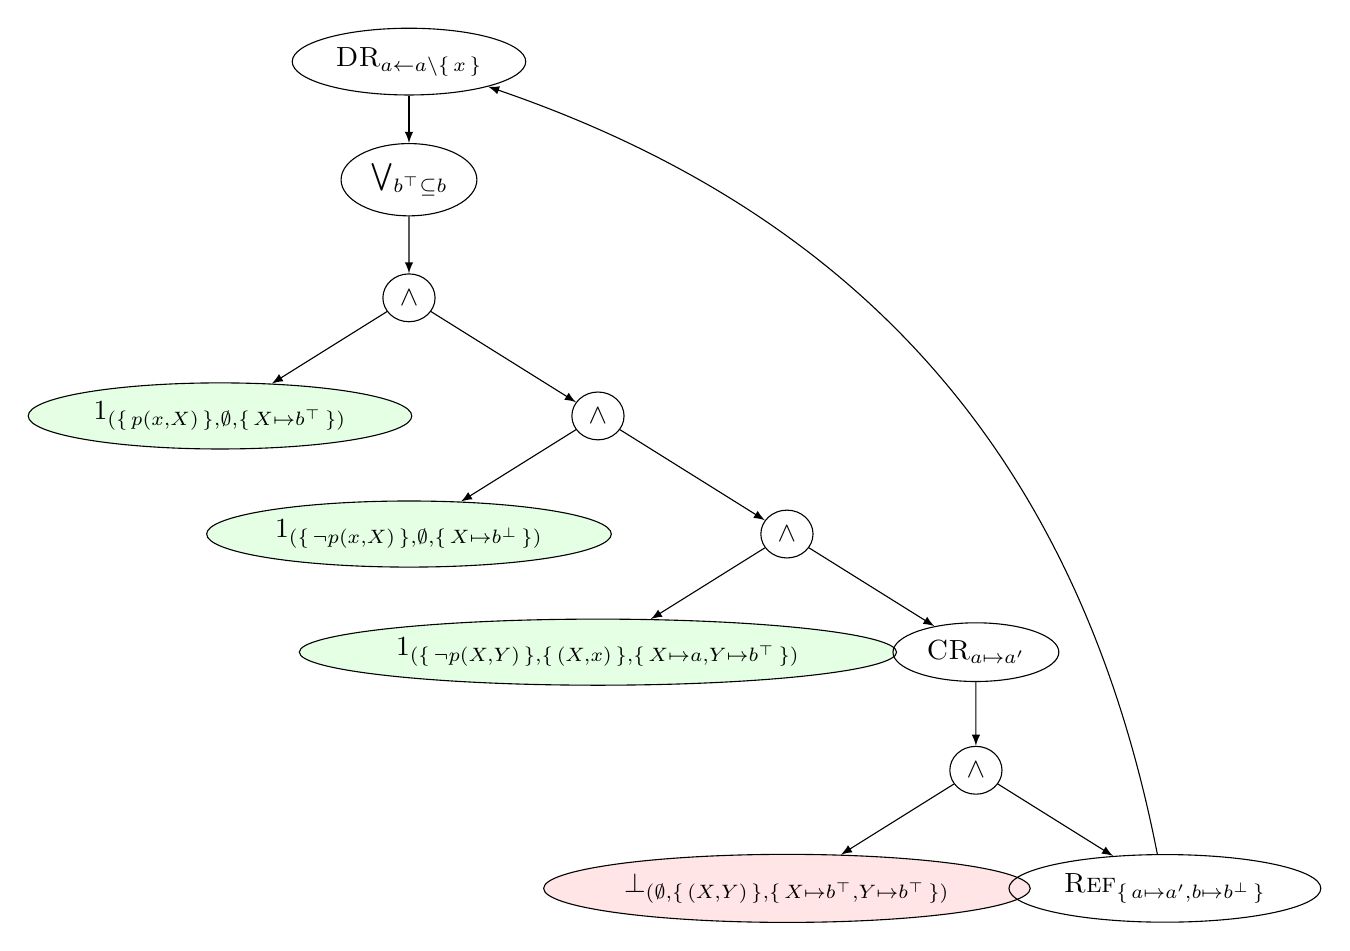
\begin{tikzpicture}[every node/.style={draw,ellipse},edge from parent/.style={draw,-latex},sibling distance=48mm]
    \node (dr) {$\DR_{a \gets a \setminus \{\, x \,\}}$}
    child {node {$\bigvee_{b^\top \subseteq b}$}
      child {node {$\wedge$}
        child {node[fill=green!10] {$1_{(\{\, p(x, X) \,\}, \emptyset, \{\, X \mapsto b^\top \,\})}$}}
        child {node {$\wedge$}
          child {node[fill=green!10] {$1_{(\{\, \neg p(x, X) \,\}, \emptyset, \{\, X \mapsto b^\bot \,\})}$}}
          child {node {$\wedge$}
            child {node[fill=green!10] {$1_{(\{\, \neg p(X, Y) \,\}, \{\, (X, x) \,\}, \{\, X \mapsto a, Y \mapsto b^\top \,\})}$}}
            child {node {$\CR_{a \mapsto a'}$}
              child {node {$\wedge$}
                child {node[fill=red!10] {$\bot_{(\emptyset, \{\, (X, Y) \,\}, \{\, X \mapsto b^\top, Y \mapsto b^\top \,\})}$}}
                child {node (ref) {$\Reff_{\{\, a \mapsto a', b \mapsto b^\bot \,\}}$}}
              }}}}}};
    \draw[-latex, bend right] (ref) to (dr);
  \end{tikzpicture}
  \caption{A graphical representation of an FCG for injections and partial injections between two domains. TODO: add a reference to a formula?}
  \label{fig:examplefcg}
\end{figure}

\paragraph{TODO.}
\begin{itemize}
\item Describe \cref{fig:examplefcg} and connect it to the algebraic formula.
\item Explain the algebraic notation that I'm using here (e.g., that $f$ is always the main function)
\item Explain the importance of comparing domain sizes to 2. FCGs that compare the size of a domain to an integer can be constructed automatically using compilation rules, although $n$ is upper bounded by the maximum number of variables in any clause of the input formula since there is no rule that would introduce new variables.
\item Mention that it only takes a few seconds to find these solutions. Going beyond depth 6 (or sometimes even completing depth 6) is computationally infeasible with the current implementation, but depth at most 5 can be searched within at most a few seconds.
\item Combine the tikz and the algebraic notation into one, so I don't need to have two versions. But how? Maybe associate a symbol with each type and only to the types that I use?
\item the exponential solutions can be computed in quadratic time with dynamic programming!
\item Can't explain how formulas are translated into (my definition of) clauses without explaining Skolemization, which is out of scope.
\item Note that in some cases different descriptions of the same problem lead to different solutions (with different complexities).
\item Maybe we are actually guaranteed that the solution is always polynomial-time. Except... running time could be infinite?
\end{itemize}

Let $p$ be a predicate of arity two s.t. the first argument is associated with domain $a$, and the second argument is associated with domain $b$ (i.e., $p$ represents a relation between sets $a$ and $b$). Then, to restrict all relations representable by $p$ to just functions from $a$ to $b$, in first-order logic one might write
\begin{gather}
  \forall X \in a. \forall Y \in b. \forall Z \in b. p(X, Y) \land p(X, Z) \implies Y = Z \label{eq:def1} \\
  \forall X \in a. \exists Y \in b. p(X, Y). \label{eq:def2}
\end{gather}
The former says that one element of $a$ can map to at \emph{most} one element of $b$, and the latter says that each element of $a$ must map to at \emph{least} one element of $b$. One might add
\begin{equation} \label{eq:injectivity}
  \forall W \in a. \forall X \in a. \forall Y \in b. p(W, Y) \land p(X, Y) \implies W = X
\end{equation}
to restrict $p$ to injections or
\begin{equation}
  \forall Y \in b. \exists X \in a. p(X, Y)
\end{equation}
to ensure surjectivity or remove \cref{eq:def2} to consider partial functions. Lastly, one can replace all occurrences of $b$ with $a$ so as to model endofunctions instead.

\paragraph{Notes.}
\begin{itemize}
\item \textsc{ForcLift} fails on all of these.
\item Functions, surjections, and their partial counterparts are/were already liftable. It seems like lifting injectivity (which is a fairly general property) is the main accomplishment. (But this is just the one I noticed. There may be many others as well.)
\item Here, $[\cdot]$ is the Iverson bracket.
\end{itemize}

\paragraph{Results.}
\begin{itemize}
\item 1d bijections and 1d injections (note that it's the same problem). Depth 3 solution:
  \begin{align*}
    f(n) &= \sum_{m=0}^n \binom{n}{m} (-1)^{n-m}g(n, m) \\
    g(n, m) &= \sum_{l=0}^n \binom{n}{l}[l < 2]g(n-l, m-1) \\
    &= g(n, m - 1) + ng(n - 1, m - 1),
  \end{align*}
  which works with base case $g(n, 0) = 1$.
\item 1d partial injections. 2 solutions at depth 6, but they're too complicated to check by hand. A contradiction with $X \ne x$ constraints makes things complicated.
\item 2d bijections. Depth 3:
  \begin{align*}
    f(m, n) &= \sum_{l=0}^m \binom{m}{l} [l < 2] (1 - [l < 1])f(m-l, n-1) \\
    &= mf(m-1, n-1),
  \end{align*}
  which works with base cases $f(0, 0) = 1$, $f(0, n) = 0$, $f(m, 0) = 0$.
\item 2d injections. Depth 2:
  \begin{align*}
    f(m, n) &= \sum_{l=0}^m \binom{m}{l}[l<2]f(m-l, n-1) \\
    &= f(m, n-1) + mf(m-1, n-1),
  \end{align*}
  which works with base cases $f(0, 0) = 1$ and $f(m, 0) = 0$.
\item 2d partial injections, depth 2. Exactly the same circuit as above but with base case $f(m, 0) = 1$.
\end{itemize}

\section{Discussion}

\begin{itemize}
\item new rules that don't create vertices (e.g., duplicate removal, unconditional contradiction detection, etc.)
\item some notes on halting
  \begin{itemize}
  \item Search is infinite. Some rules increase the size of the formula(s), but most reduce it.
  \item Inference is guaranteed to terminate if at least one domain shrinks by at least one. But note that allowing recursive calls with the same domain sizes (e.g., $f(n) = f(n) + \dots$) could be useful because these problematic terms might cancel out.
  \item It's impossible for $n \gets n - 1$ and $\texttt{for } n \in \dots$ to combine in a way that results in an infinite loop.
  \end{itemize}
\item care should be taken when cloning to preserve the validity of the cache and avoid infinite cycles (we use a separate (node $\to$ node) cache for this)
\end{itemize}

\section{Conclusions and Future Work}

\paragraph{Conclusions and observations.}
\begin{itemize}
\item $\CR$ must be separate from $\DR$ because initially the requirement to not have the newly introduced constant in the literals is not satisfied.
\end{itemize}

\paragraph{Future work.}
\begin{itemize}
\item Transform FCGs to definitions of (possibly recursive) functions on integers. Use a computer algebra system to simplify them.
\item Design an algorithm to infer the necessary base cases. (Note that there can be an infinite amount of them when functions have more than one parameter.)
\item Observation: -1 (and powers thereof) appear in every solution to a formula if and only if the formula has existential quantification. That's not very smart! By putting unit propagation into $\Gamma$, these powers are pushed to the outer layers of the solution (i.e., `early' in the FCG). It's likely that removing this restriction would enable the algorithm to find asymptotically optimal solutions.
\end{itemize}

\bibliographystyle{acm}
\bibliography{notes}

\end{document}
